\documentclass[11pt,a4paper]{article}
\usepackage[margin=24mm]{geometry}
\usepackage{amsmath,amssymb,graphicx,longtable,array}
\newcommand{\E}{\mathbb E}
\newcommand{\Var}{\operatorname{Var}}
\newcommand{\Cov}{\operatorname{Cov}}
\newcommand{\MSE}{\operatorname{MSE}}
\newcommand{\RMSE}{\operatorname{RMSE}}
\setlength{\parskip}{4pt}
\setlength{\parindent}{0pt}
\renewcommand{\arraystretch}{1.12}
\emergencystretch=2em
\newcommand{\MatchedBaseRMSE}{0.0927}
\newcommand{\MatchedRMSE}{0.0244}
\newcommand{\MatchedCoverage}{94.6}
\newcommand{\MatchedMSEReduction}{93.1}
\newcommand{\ProfileBaseRMSE}{0.0454}
\newcommand{\ProfileRMSE}{0.0238}
\newcommand{\ProfileCoverage}{94.3}
\newcommand{\ReverseRMSE}{0.1809}
\newcommand{\ReverseResidualRMSE}{0.0239}
\newcommand{\ReverseResidualCoverage}{94.9}
\newcommand{\DoubleCoverage}{5.3}

\title{When does orienting negative controls help?\\A binary-outcome benchmark for educational data}
\author{Research supplement to the working manuscript}
\date{29 October 2026}
\begin{document}
\maketitle
\begin{abstract}
Sign alignment prevents cancellation among negative-control estimates, but does not establish that their average measures the bias of a different outcome. We isolate these issues using 58 prospectively specified binary-risk scenarios with 1000 independent training/evaluation replications each. The experiments separate loading mismatch, weak proxy information, incompatible hidden factors, invalid controls and observed-stratum reversal of proxy associations. A second benchmark uses the joint baseline distribution of 5823 OULAD training students, with generated treatments and outcomes of known effect. With matched loadings and an informative proxy, the original correction reduces RMSE from \MatchedBaseRMSE{} to \MatchedRMSE{}, with \MatchedCoverage\% nominal interval coverage. When the control loading doubles, coverage falls to \DoubleCoverage\%; stratum-induced sign reversal can make correction substantially worse. Residual orientation repairs that particular reversal but does not solve factor or scale mismatch. We derive the correction's bias in an explicit additive binary-risk model and provide a conditional finite-sample interval under known marginal propensity and a justified structural bias bound. This elementary result is deliberately distinguished from the historical MoM interval and from feasible inference with unknown mismatch. The contribution is a reproducible educational benchmark and a sharper account of applicability, not a claimed new causal-identification method.
\end{abstract}

\section{Contribution and relation to the manuscript}

The editor identified two separate issues: orientation is a simple coding operation, and the controls may not be commensurable with the target's confounding bias. This supplement addresses the second issue directly and narrows the first claim. It retains the original equal-weight correction as the object of evaluation. Candidate alternatives are explicitly labelled ablations or comparators, rather than silently replacing the retained method.

The new research question is: under what combinations of orientation reliability, loading similarity and shared confounding does a sign-aligned panel improve a target estimate? Three kinds of evidence are separated: known-truth structural simulations, an OULAD-profile simulation with artificial responses, and previously recomputed observational OULAD/XES diagnostics. The first two permit measurement of estimation error. The third does not supply the true target effect.

The original manuscript and its abstract were not regenerated in this run. This standalone supplement can be reviewed alongside that draft; its proposed contribution statement appears in Section~\ref{sec:contribution}. It does not certify submission readiness or resolve the empirical comparability of the original OULAD panel.

\section{What is already known}

COCA already develops causal correction through negative-control outcomes, including binary settings and imperfect controls \cite{coca}. Single-proxy work establishes identification under specific counterfactual assumptions rather than a sign convention \cite{park}. Equi-confounding and its failure are established issues \cite{caveats}. Accordingly, the existence of a residual-bias expression below is not itself a novelty claim.

Empirical confidence-interval calibration uses a distributional systematic-error model and negative plus synthetic positive controls \cite{schuemie}. It does not require every control to have the same bias magnitude. Our unsigned MoM and random-effects comparators are therefore not labelled full replications of that procedure. Earlier binary simulations already contrast suitable and unsuitable controls \cite{hwang}. Multi-outcome sensitivity analysis uses factor structure and null controls to bound causal effects \cite{zheng}. More recent NC-DiD uses multiple controls, including median aggregation, in a pre/post design \cite{ncdid}; the 2026 distributional-calibration preprint includes panel diagnostics and leave-one-out evaluation \cite{dc}. Leave-one-out checking, median pooling and sensitivity intervals cannot independently support priority claims here.

The specific empirical addition is a decomposition of the retained orientation rule's failure modes under common adjustment, independent sign estimation and educational baseline distributions. The bibliography is a targeted comparison, not a systematic search proving that this precise benchmark has no predecessor.

\section{An explicit binary-risk model}

Let $Z$ denote finitely many observed strata with probabilities $p_z$, $U$ a bounded latent vector, $A$ a binary treatment, $Y$ a binary target and $C_k$ binary candidate controls. Assume consistency and independence of assignment and potential-response errors conditional on $(Z,U)$. Consider
\begin{align}
 \E[Y(a)\mid z,u]&=m(z)+\tau(z)a+\lambda_Y(z)'u,\\
 \E[C_k(a)\mid z,u]&=c_k(z)+\gamma_k(z)a+\lambda_k(z)'u.
\end{align}
All response probabilities must lie in $[0,1]$. A valid negative control has $\gamma_k(z)=0$. The model is additive on the probability scale; it is not a logistic model, and its conclusions cannot simply be transferred to odds ratios. The population target is $\theta=\sum_zp_z\tau(z)$.

Define $\Delta(z)=\E[U\mid A=1,z]-\E[U\mid A=0,z]$. The standardized observed contrasts obey
\begin{align}
 d_Y&=\theta+\sum_zp_z\lambda_Y(z)'\Delta(z),\\
 d_k&=\sum_zp_z\{\gamma_k(z)+\lambda_k(z)'\Delta(z)\}.
\end{align}
Thus exclusion of a causal treatment effect on a control and comparability of confounding bias are distinct restrictions.

\subsection{Bias after orientation}

Condition on an independent training sample $D$. Let $s_k(D)\in\{-1,1\}$ and $w_k(D)\ge0$, $\sum_kw_k(D)=1$. The retained procedure uses $w_k=1/K$. For $q_s=d_Y-\sum_kw_ks_kd_k$, substitution gives the exact identity
\begin{equation}\label{eq:bias}
q_s-\theta=\sum_zp_z\left[\left\{\lambda_Y(z)-\sum_kw_ks_k\lambda_k(z)\right\}'\Delta(z)-\sum_kw_ks_k\gamma_k(z)\right].
\end{equation}
In a correctly oriented one-factor model with valid controls and constant loadings this reduces to $(\lambda_Y-\sum_kw_k|\lambda_k|)\Delta$. Correcting the signs does not establish equality of the target and control loadings.

Writing $B=d_Y-\theta$ and $M=\sum_kw_ks_kd_k$, the reduction in squared population bias is $2BM-M^2$. If $B\ne0$, its positivity requires $0<M/B<2$. At finite sample size the full random correction $C$ and initial estimator $T$ instead satisfy
\begin{equation}
\MSE(T)-\MSE(T-C)=2B_T\mu-\mu^2-\Var(C)+2\Cov(T,C),
\end{equation}
where $B_T=\E[T]-\theta$ and $\mu=\E[C]$. This standard identity includes training-sign randomness and explains why scale matching and variance both matter.

\subsection{A structural mismatch allowance}

Suppose scientific information supplies coordinatewise restrictions
\begin{align*}
 \left|\lambda_{Y,j}(z)-\sum_kw_ks_k\lambda_{k,j}(z)\right|&\le\epsilon_j(z),\\
 |\Delta_j(z)|&\le D_j(z),\qquad |\gamma_k(z)|\le\Gamma_k(z).
\end{align*}
Equation~\eqref{eq:bias} implies, by the triangle inequality,
\begin{equation}\label{eq:bound}
 |q_s-\theta|\le R_s:=\sum_zp_z\left\{\sum_j\epsilon_j(z)D_j(z)+\sum_kw_k\Gamma_k(z)\right\}.
\end{equation}
The restrictions refer to differences in response-risk gradients, latent selection and exclusion validity. They are not estimated by observing that the control estimates have similar signs. For scalar $U\in[-1,1]$, a loading mismatch of .03 permits a target/control difference of .06 in the risk change across the full latent range.

If matching is assumed for a reference orientation $s^*$ but an estimated sign is wrong, a sufficient replacement for $\epsilon_j(z)$ is
\[
 \epsilon_j(z)+2\sum_{k:s_k\ne s_k^*}w_kL_{kj}(z),
 \qquad |\lambda_{k,j}(z)|\le L_{kj}(z).
\]
This follows by adding and subtracting the reference pool. Weak proxy evidence cannot justify omitting that additional term. For training-estimated weights, the restriction must hold for the selected weights, or uniformly over possible training selections. Unknown allowances remain sensitivity assumptions.

\subsection{What the original summaries do not identify}

Take $U=\pm1$ with equal probabilities, $P(A=1\mid U)=.5+.15U$, and $\E[C_k\mid U]=.5+.14s_kU$ with alternating $s_k$. Let $G=U+$ independent noise and $\E[Y(a)\mid U]=.5+\tau(a-.5)+\lambda U$. Two admissible models have $(\tau,\lambda)=(0,.14)$ and $(.042,.07)$. In both, $d_Y=\tau+.60\lambda=.084$ and every correctly oriented control contrast equals $.084$. The marginal arm risks and variances and proxy-orientation signs also agree. The original population MoM correction is zero in both, despite different true effects.

This is equivalence of summaries retained by the original pooling procedure, not equivalence of the full observed joint distribution: target/control cross-covariances can differ. It shows why these summaries alone do not identify the causal correction. The example is explanatory and carries no claim of a new general nonidentification theorem.

\section{A conditional finite-sample result and its limits}

Assume $D$ is independent of $n$ iid evaluation observations. Let the marginal propensity $e(z)=P(A=1\mid Z=z)$ be known, with $\eta\le e(z)\le1-\eta$ for known $\eta>0$. Freeze $s,w$ after training, and set
\begin{align*}
 V_i&=Y_i-\sum_kw_ks_kC_{ik},\\
 H_i&=\frac{A_iV_i}{e(Z_i)}-\frac{(1-A_i)V_i}{1-e(Z_i)},\\
 M_s&=1+\sum_{k:s_k=-1}w_k,\qquad
 r_n=\frac{2M_s}{\eta}\sqrt{\frac{\log(2/\alpha)}{2n}}.
\end{align*}
\textbf{Proposition.} If a training-measurable $R_s$ bounds $|q_s-\theta|$ almost surely, then
\[
 I=[\bar H-r_n-R_s,\ \bar H+r_n+R_s]\cap[-1,1]
\]
has conditional and unconditional coverage at least $1-\alpha$.

\textit{Proof.} Conditional on $D$, $\E[H_i\mid D]=q_s$. Binary responses and simplex weights imply $-\sum_{s_k=1}w_k\le V_i\le1+\sum_{s_k=-1}w_k$, hence $H_i\in[-M_s/\eta,M_s/\eta]$. Hoeffding's inequality \cite{hoeffding} gives $P(|\bar H-q_s|>r_n\mid D)\le\alpha$. On its complementary event, the triangle inequality yields $|\bar H-\theta|\le r_n+R_s$. Intersecting with the binary-ATE space preserves coverage. Integrating over $D$ proves the unconditional claim. If the structural bound holds only on a training event with probability at least $1-\beta$, the union-bound guarantee becomes $1-\alpha-\beta$.

This is an elementary concentration-and-sensitivity result, not an asserted novel interval method. Estimated training signs and simplex weights are permitted because they are frozen before evaluation, but estimated propensity scores, unknown $R_s$, same-sample selection and population transport are not solved by this proof. In the benchmark, $R_s$ is computed from the true simulated loadings and latent selection, labelled \emph{oracle structural bound}. Its coverage cannot be represented as evidence that a feasible procedure learned the unknown target bias from the controls.

The historic MoM interval is a different construction. A covariance-aware Wald interval plus a fixed $R$ is also reported as an asymptotic sensitivity display, not an instance of the finite-sample proposition. Neither construction inherits its guarantee merely by widening an estimated-propensity AIPW interval from the real-data audit.

\section{Experiment design}

The local protocol was written before executing these experiments, after the earlier editorial audit; it is not an external preregistration. All 58 specified cells and all adverse results were retained. Each uses 1000 replications, a new independent training sample of 1000 units in every replication, and an evaluation sample of 2000 unless stated otherwise. No treatment-by-stratum cell failed; no redraws were used to hide failures.

\subsection{Known truth and empirical educational structure}

The synthetic population crosses $Z\in\{0,1,2\}$ with two independent symmetric latent coordinates $U_j=\pm1$. The marginal treatment probabilities are $(.35,.50,.65)$, and the conditional assignment is $e(Z)+a'\{U-\E[U\mid Z]\}$. Usually $a=(.15,0)'$. The target probability is $.45+.05(Z-1)+\tau A+\lambda_Y'U$, with $\tau\in\{0,.08\}$ and usually $\lambda_Y=(.14,0)'$. The six control loadings alternate in sign, with magnitude $r\lambda_Y$ in the matched-factor grid. Independent response errors are generated for each outcome. Probabilities are validated rather than clipped.

The proxy is $G=\rho\{U_1-\E(U_1)\}/\operatorname{sd}(U_1)+\sqrt{1-\rho^2}N$, with $N$ independent standard normal. The grid uses $r\in\{.25,.5,1,1.5,2\}$, $\rho\in\{0,.25,.75\}$, and two effects: 30 synthetic cells. Four additional sample-size cells use $n=500$ or $8000$ at $r=1,\rho=.25$. Two no-confounding cells use $a=0$.

The OULAD-profile population uses 5823 unique training students from OULAD \cite{oulad}, obtained by merging archived training registration keys with the processed student table and deterministic student deduplication. Credits define strata $<60$, $60$--$119$, and $\ge120$. Age codes are $-1,.4,1$ for the three released age groups; previous attempts define a second $\pm1$ coordinate. These are simulation choices, not validated latent educational constructs. Twelve cells cross $r\in\{.5,1,2\}$, $\rho\in\{.25,.75\}$ and the two effects. Evaluation units are independent draws with replacement from this fixed empirical population. Treatments, proxies and responses are generated: the true effect of an actual educational intervention is not known from these data. The proxy coefficient need not equal its observed correlation in this empirical population.

\subsection{Mechanism stresses}

Ten cells isolate five failures at $\rho=.75$ and both effects. \emph{Second-factor} controls depend on $U_2$, while assignment and target depend on $U_1$. \emph{Opposed-factor} controls have loadings proportional to $(-.14,.28)'$, the target to $(.07,.07)'$, and assignment depends on both latent coordinates. The proxy tracks $U_1$, so orienting by it can reverse the relevant combined selection bias. \emph{Invalid-control} cases add a direct treatment risk difference of .12 to one or two positively loaded controls. \emph{Stratum reversal} adds $2(Z-1)$ to the proxy and control intercept trends $-.22s_k(Z-1)$: marginal proxy associations can then have the opposite sign to the hidden-factor loadings.

\subsection{Estimators and reporting}

All outcomes share saturated standardization over the same three observed strata and known population stratum weights. Joint outcome influence scores provide covariance-aware standard errors. This structural benchmark does not reproduce the earlier machine-learning nuisance design, and the evaluation adjustment set contains $Z$, not the training-only proxy. It deliberately isolates an underadjusted contrast to examine correction.

Raw orientation uses target/proxy and control/proxy covariance signs estimated in the independent training sample. Residual orientation first removes training stratum means from the proxy and outcomes; it is an established residualization ablation, not a claimed new causal method. True-loading orientation and IPW using the full hidden assignment probability are unavailable-information oracle benchmarks. Other comparisons are unsigned pooling, conventional inverse-variance random-effects pooling and an oriented median point estimate. The median has no reported confidence interval and is not described as NC-DiD. The random-effects comparator is not the full Schuemie positive-control procedure.

Sixteen reported method/interval variants include the original MoM interval, shared-score Wald variants, fixed allowances $R\in\{.025,.05,.10,.20\}$ and the oracle-bound finite-sample interval. Adding $R$ changes interval width, not the corrected point estimate. Bias, RMSE, coverage, rejection probability and width are stored for all 928 scenario-method combinations; all 928000 replicate estimates are archived in compressed form. Rejection is type I error at $\tau=0$ and power at $.08$. Paired MSE comparisons include pointwise Monte Carlo uncertainty; they are descriptive comparisons across a designed grid, not a multiple-testing certification of universal superiority. At coverage .95 the Monte Carlo standard error is approximately .0069 with 1000 replications.

\section{Results}

\subsection{Matching helps, but reliable signs do not repair scale mismatch}

With $r=1,\rho=.75,\tau=0$, the original correction reduces RMSE from \MatchedBaseRMSE{} to \MatchedRMSE{} and MSE by \MatchedMSEReduction\%, with \MatchedCoverage\% coverage. This is a condition-matched result, not an average benefit for educational studies. When $r=2$, coverage is only \DoubleCoverage\%, although the proxy remains informative. Increasing sign reliability can expose systematic overcorrection rather than repair it (Figure~\ref{fig:grid}). At $r=.5$, point error can improve while interval coverage remains poor. Error reduction and valid inference must therefore be assessed separately.

\begin{figure}[htbp]
\centering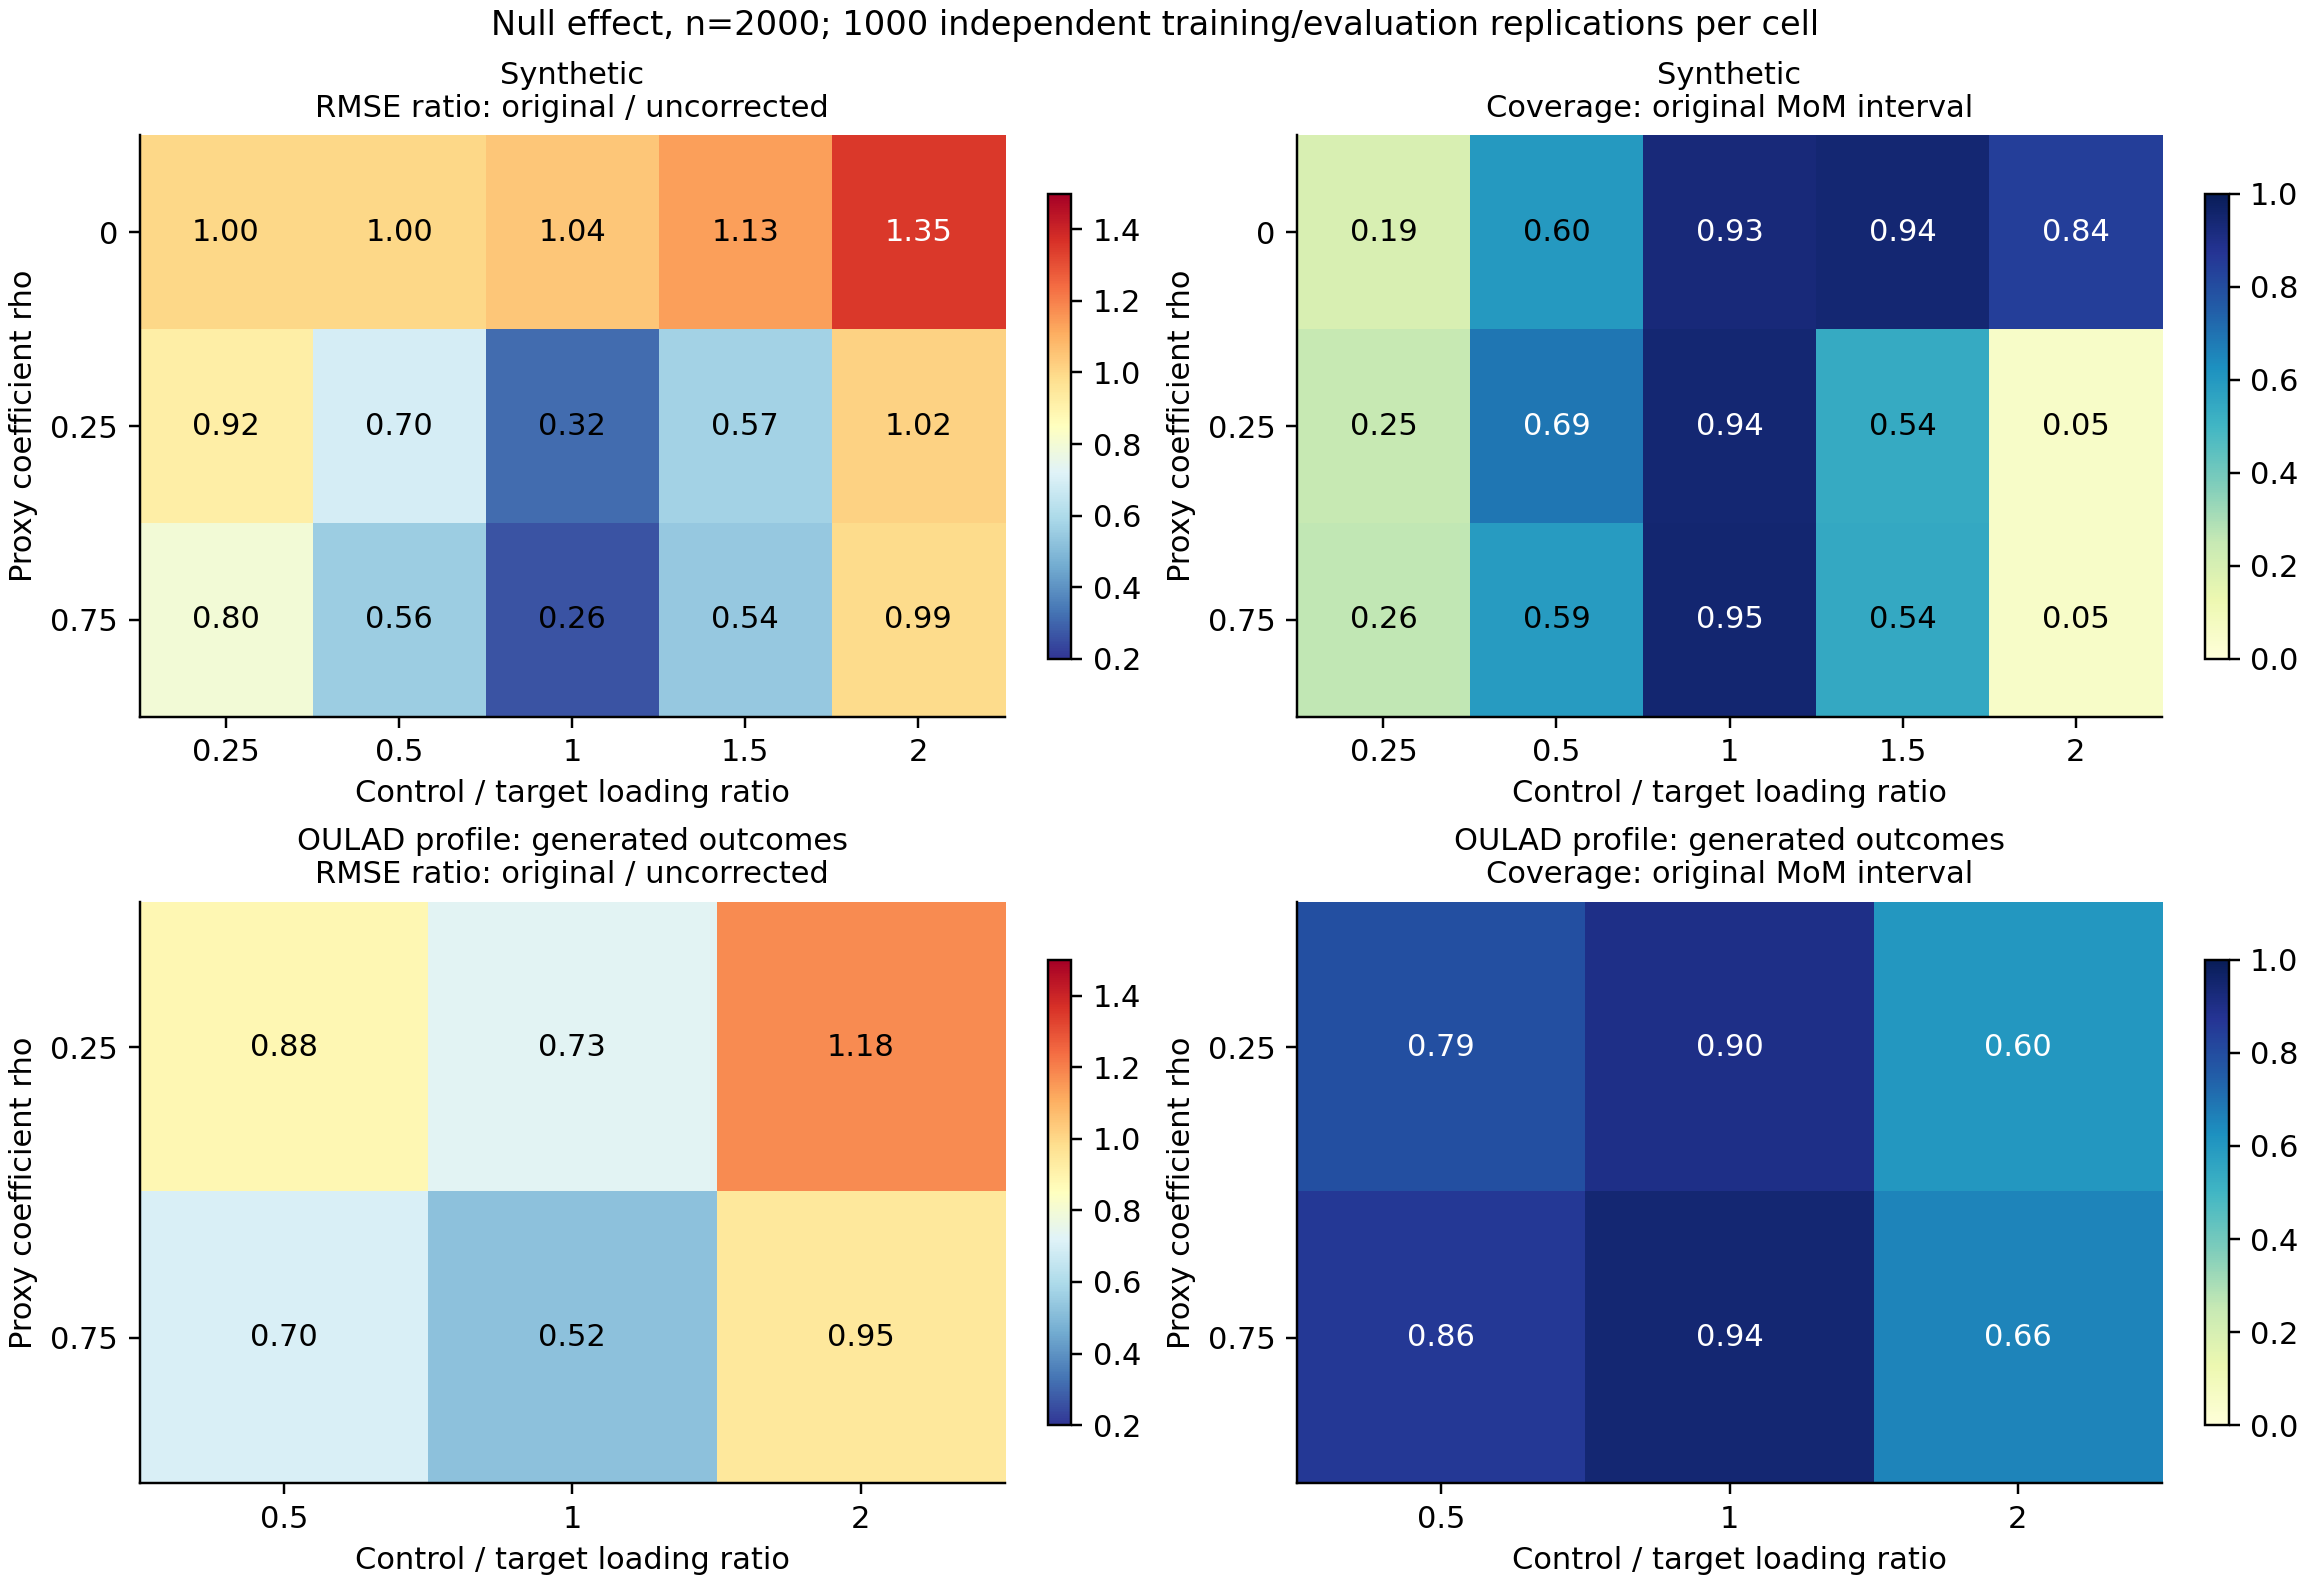
\includegraphics[width=\textwidth]{grid.png}
\caption{Complete null-effect scale/proxy grids. Ratios below one indicate lower RMSE than the uncorrected estimator. The OULAD rows use generated outcomes and preserve only an empirical baseline distribution. Every cell has 1000 replications; alternative-effect results are included in Table~\ref{tab:all}.}\label{fig:grid}
\end{figure}

At $\rho=0$, higher apparent MoM coverage in some cells accompanies increased dispersion and can coexist with worse point estimates. This is not successful bias learning. Without hidden confounding, adding noisy controls also needlessly increases point-estimation error. Across the entire designed grid, the paired MSE difference favours the original procedure in 33 cells, disfavors it in 14, and is inconclusive in 11 at the pointwise Monte Carlo interval criterion. These counts depend on the chosen grid and are not probabilities of success in applications.

\subsection{Residual orientation repairs one failure, not comparability}

The stratum-reversal stress increases original-method RMSE to \ReverseRMSE{}. Residual orientation reduces it to \ReverseResidualRMSE{} with \ReverseResidualCoverage\% coverage. Both procedures retain the same equal pooling: the change isolates an orientation problem. Residualization does not repair second-factor controls or the opposed-factor construction, because those panels do not measure target bias on the necessary scale. Treating the residualization improvement as a general new calibration method would repeat the editor's concern.

\begin{table}[htbp]
\centering\small
\caption{Mechanism-specific comparisons at $\tau=0$, $\rho=.75$, $n=2000$. ``Residual'' changes the training orientation rule only. Coverage is for the corresponding MoM interval.}
\begin{tabular}{lrrrrr}\hline
 & Raw RMSE & Original RMSE & Cover. & Residual RMSE & Cover.\\\hline
Matched controls & 0.0927 & 0.0244 & 0.946 & 0.0244 & 0.946 \\
Second factor & 0.0927 & 0.0931 & 0.061 & 0.0930 & 0.059 \\
Opposed factors & 0.0504 & 0.0942 & 0.062 & 0.0942 & 0.062 \\
One invalid & 0.0927 & 0.0312 & 0.999 & 0.0312 & 0.999 \\
Two invalid & 0.0927 & 0.0463 & 1.000 & 0.0463 & 1.000 \\
Stratum reversal & 0.0927 & 0.1809 & 0.000 & 0.0239 & 0.949 \\
No confounding & 0.0225 & 0.0235 & 0.956 & 0.0235 & 0.956 \\
\hline\end{tabular}

\end{table}

\begin{figure}[htbp]
\centering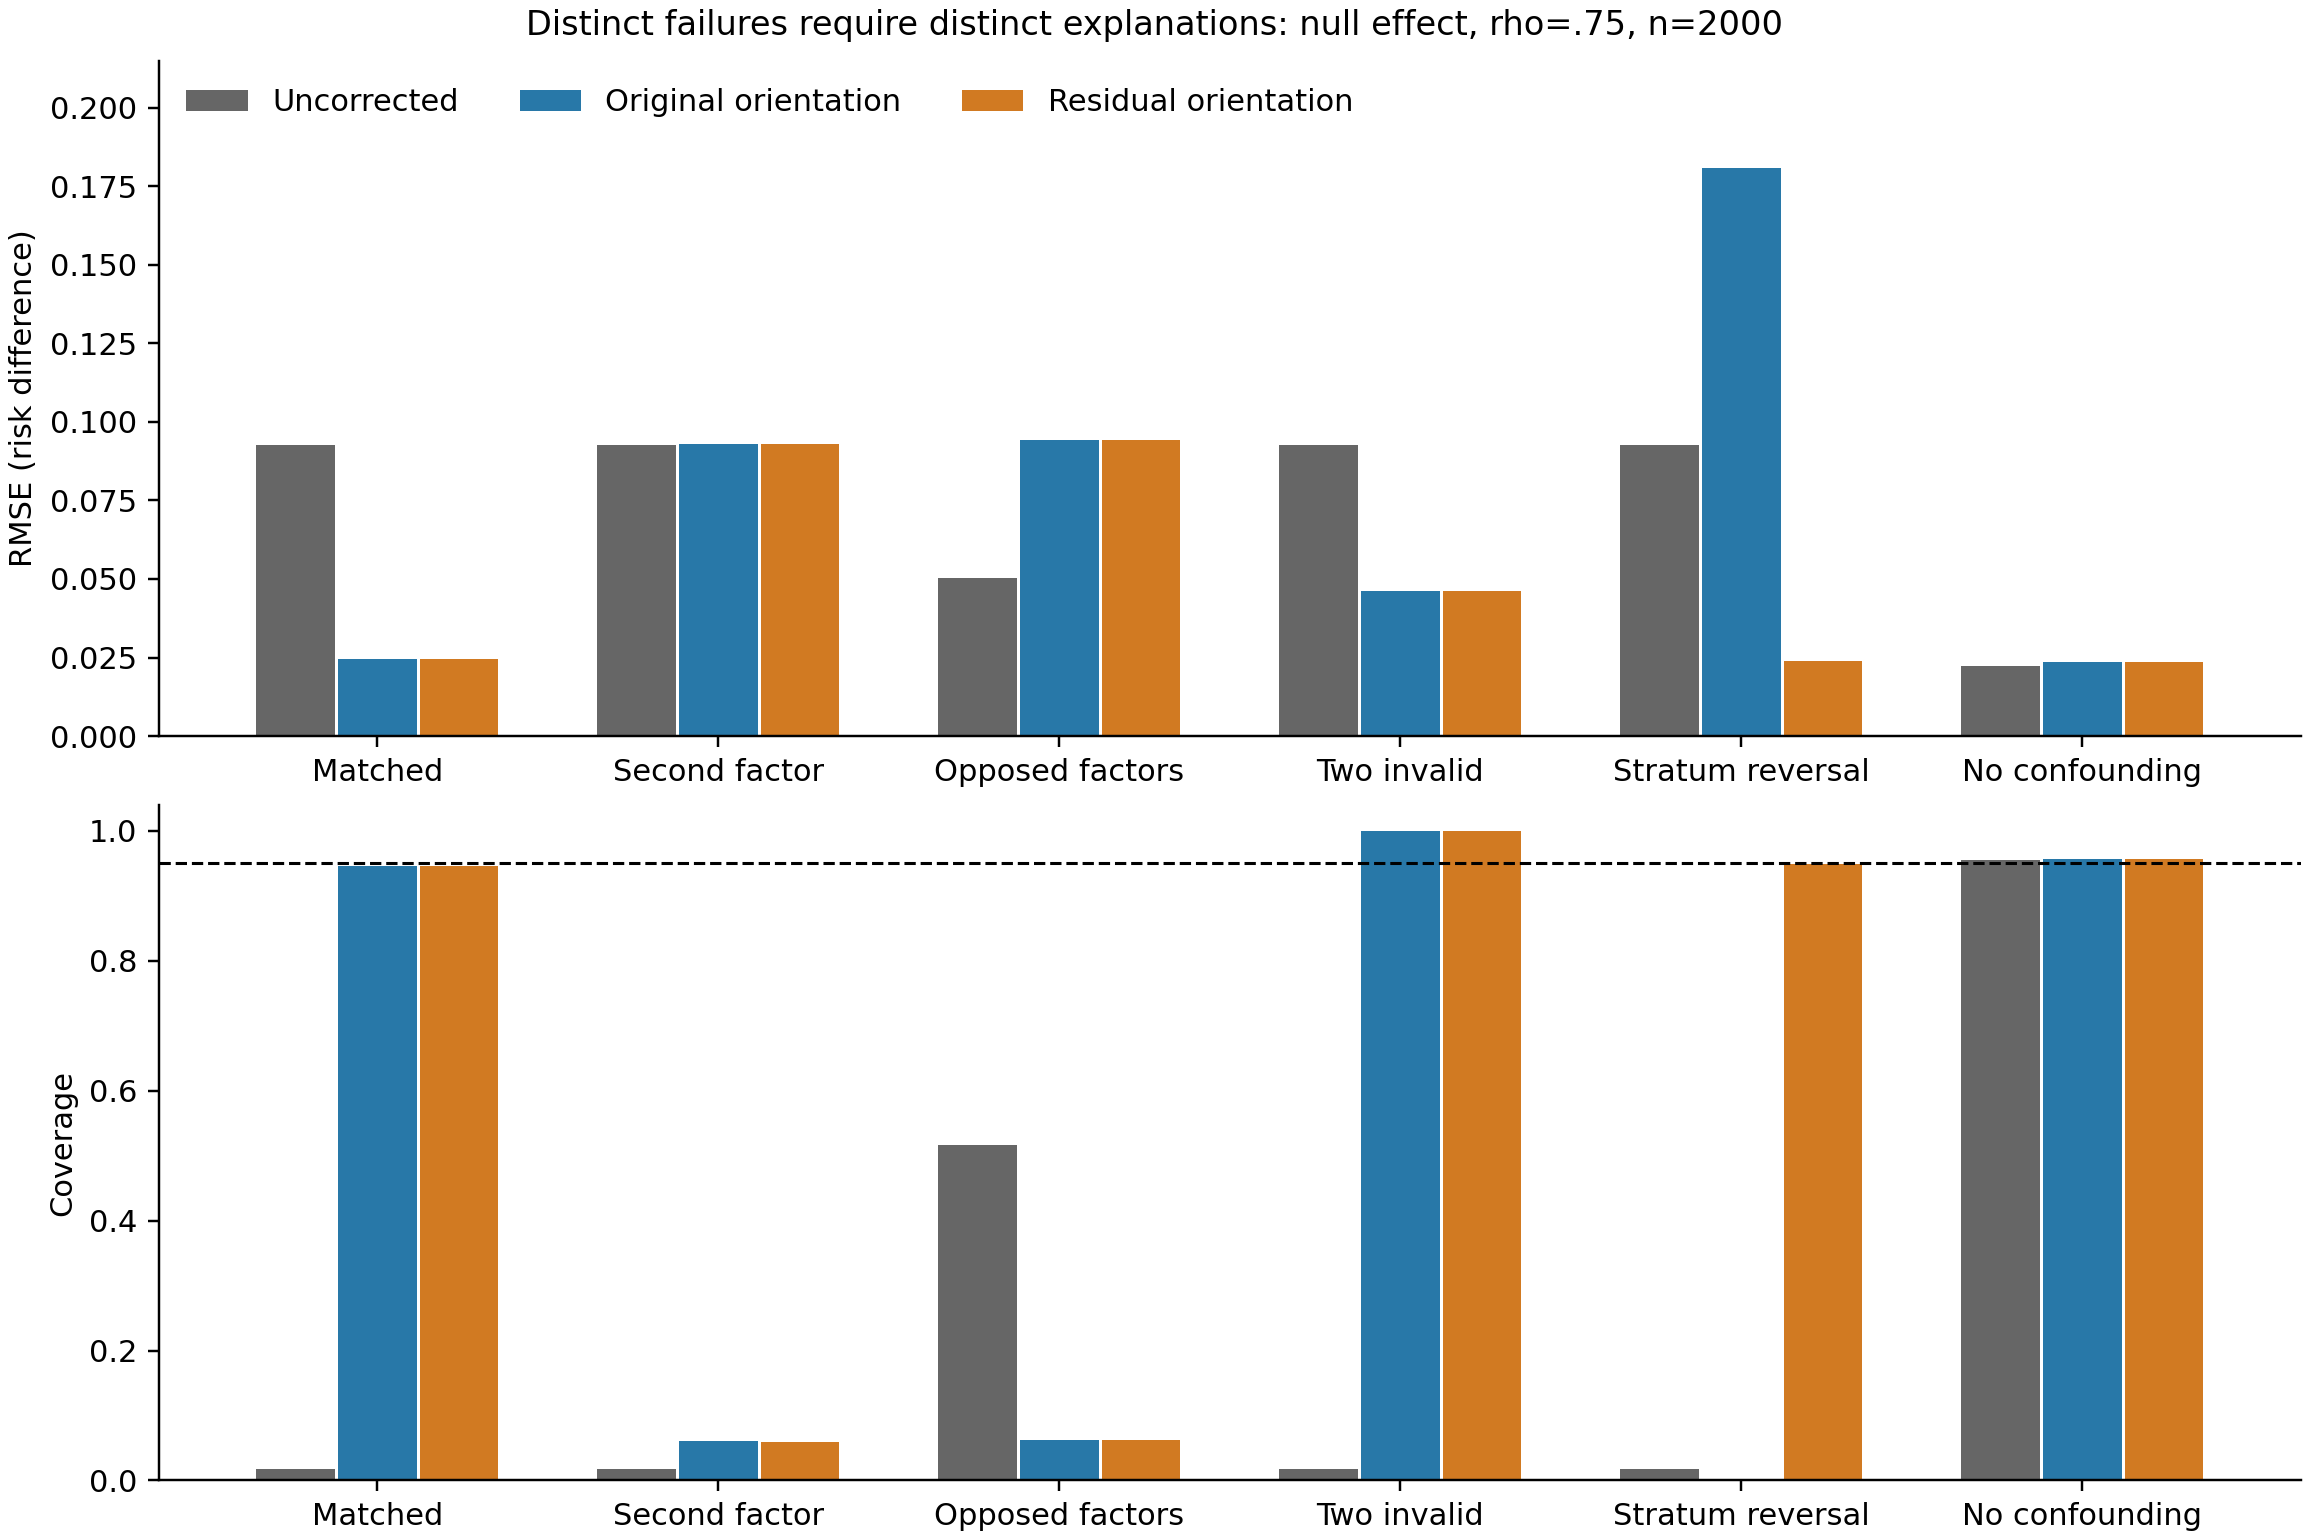
\includegraphics[width=\textwidth]{failures.png}
\caption{Point-estimation and interval performance answer different questions. Very wide intervals for invalid controls can achieve high coverage despite biased estimates. Residual orientation fixes the constructed stratum reversal but leaves incompatible-factor failures.}\label{fig:failures}
\end{figure}

\subsection{Educational-profile benchmark and real-data distinction}

Under matched loadings and $\rho=.75$, OULAD-profile RMSE decreases from \ProfileBaseRMSE{} to \ProfileRMSE{}, with \ProfileCoverage\% coverage. Weak proxy information and doubled loadings degrade these results. This constitutes known-truth evidence conditional on an empirical educational baseline distribution and synthetic response mechanisms. It does not validate the original real demographic controls or establish the true effect of on-time submission on retention.

The earlier real-data audit remains relevant as a falsification exercise: OULAD leave-one-control-out null-reference RMSE worsened from .0391 to .0447, while the XES diagnostics improved. These figures are observational checks under the previously documented common-adjustment design, not replications of this structural benchmark. XES fractional windows and the small related prefix-control panel remain limitations. Neither real audit estimates the unknown target bias directly.

\subsection{Coverage under a bias allowance has a price}

Figure~\ref{fig:sensitivity} displays fixed allowances added to the covariance-aware Wald interval. Small allowances can be adequate for matched panels and inadequate for severe sign reversal. The analyst cannot select a favorable allowance after observing simulated truth and call the result feasible inference.

\begin{figure}[htbp]
\centering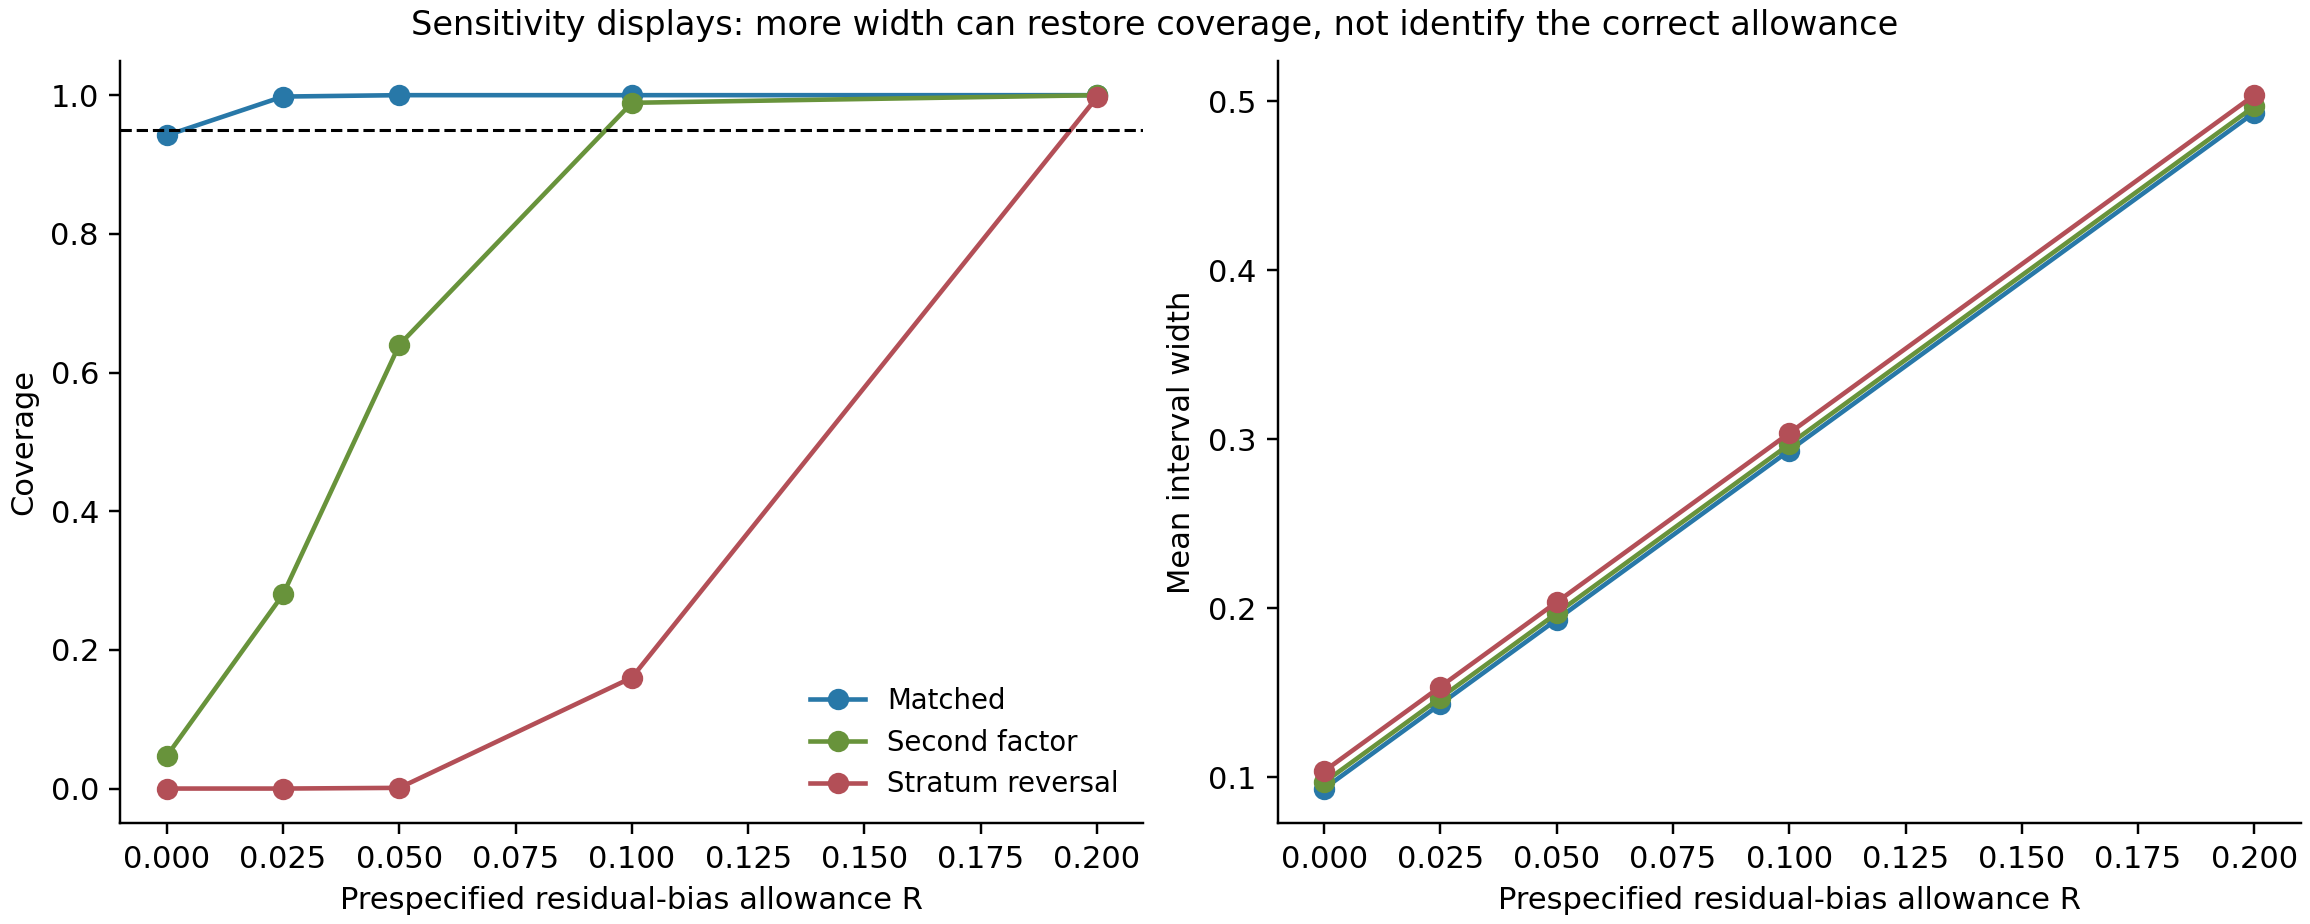
\includegraphics[width=\textwidth]{sensitivity.png}
\caption{Sensitivity intervals at $\tau=0$, $\rho=.75$, $n=2000$. The allowance is prespecified and is not learned from controls. More width can improve coverage without improving point error or establishing the assumption.}\label{fig:sensitivity}
\end{figure}

The finite-sample oracle-bound intervals cover in all 1000 replications in every cell, consistent with a conservative lower coverage guarantee. Their mean untruncated widths range from .268 to 1.053 across cells, far wider than the matched original MoM interval (about .098). This is a cost of conservative sampling bounds and explicit mismatch allowance, not increased efficiency. Its assumptions include known marginal propensity and a structurally justified bound; no such guarantee is transferred to real-data AIPW estimates.

\section{What this establishes for novelty}\label{sec:contribution}

The results support the following scoped contribution statement:

\begin{quote}
We provide a reproducible evaluation of sign-oriented negative-control pooling for educational causal analyses. An explicit binary-risk model and independent-training benchmarks separate direction errors, mismatch in bias magnitude and incompatible confounding factors. An OULAD-profile benchmark with known generated effects links these mechanisms to an empirical educational baseline distribution. The analysis shows that successful orientation and within-panel diagnostics do not establish target-bias comparability, and distinguishes nominal calibration intervals from inference conditional on a stated residual-bias allowance.
\end{quote}

This statement claims a specific empirical and explanatory contribution. It does not claim the first binary negative-control method, the first sensitivity interval, or methodological priority for simple sign alignment, residualization, median pooling, or the Hoeffding proposition. The closest existing methods are not all implemented here; no superiority over COCA, proximal inference, NC-DiD or full empirical CI calibration is established.

The principal unresolved methodological task remains to obtain defensible information about target/control mismatch and derive useful inference when nuisance functions and proxy relations are estimated. Merely assuming a small mismatch or plotting wider intervals does not solve this task. Approximate transport across distinct populations is also outside the present theorem. The educational case-study contribution is strengthened; acceptance and a new methodological gap remain unconfirmed.

\section{Reproducibility and manuscript integration}

The package includes the prospective local protocol, exact model derivation and proofs, source and input hashes, population aggregates, seed, all replicate estimates, scenario summaries, Monte Carlo errors and plotting code. No individual student records are distributed. There were 58000 successful evaluation replications and zero recorded cell failures. Structural identities were independently checked against enumeration of the finite populations for all 58 scenarios and three orientations, giving 174 checks.

For integration, the contribution statement belongs in the introduction; the binary model and separation of sign versus magnitude assumptions belong in Methods; Figures~\ref{fig:grid}--\ref{fig:sensitivity} and the full cell table belong in Results or supplementary material; the known-propensity proposition should remain a clearly qualified appendix result. The old abstract was not regenerated, and the supplement does not authorize claiming that the original OULAD comparability objection is resolved. A new submission should retain unfavorable evidence and describe the real-data and generated-outcome designs separately.

\clearpage
\appendix
\section{All prespecified scenario cells}
\small
\setlength{\tabcolsep}{3pt}
\begin{longtable}{lp{2.5cm}rrrrrrrr}
\caption{Every prespecified cell. S=synthetic, O=OULAD-profile generated outcomes; $r$=control loading scale, $\rho$=proxy coefficient, $\tau$=true ATE. U=uncorrected RMSE; Sgn=original oriented RMSE; C=original MoM coverage; Res=residual-orientation RMSE. Each row contains 1000 replications.}\label{tab:all}\\
\hline Source & Family & $r$ & $\rho$ & $\tau$ & $n$ & U & Sgn & C & Res\\\hline
\endfirsthead
\hline Source & Family & $r$ & $\rho$ & $\tau$ & $n$ & U & Sgn & C & Res\\\hline
\endhead
\hline\endfoot
S & Scale/proxy & 0.25 & 0 & 0 & 2000 & 0.093 & 0.093 & 0.192 & 0.093 \\
S & Scale/proxy & 0.25 & 0 & 0.08 & 2000 & 0.093 & 0.093 & 0.185 & 0.093 \\
S & Scale/proxy & 0.25 & 0.25 & 0 & 2000 & 0.093 & 0.085 & 0.249 & 0.085 \\
S & Scale/proxy & 0.25 & 0.25 & 0.08 & 2000 & 0.093 & 0.086 & 0.242 & 0.086 \\
S & Scale/proxy & 0.25 & 0.75 & 0 & 2000 & 0.093 & 0.074 & 0.261 & 0.074 \\
S & Scale/proxy & 0.25 & 0.75 & 0.08 & 2000 & 0.093 & 0.075 & 0.267 & 0.075 \\
S & Scale/proxy & 0.5 & 0 & 0 & 2000 & 0.093 & 0.093 & 0.596 & 0.093 \\
S & Scale/proxy & 0.5 & 0 & 0.08 & 2000 & 0.093 & 0.094 & 0.591 & 0.094 \\
S & Scale/proxy & 0.5 & 0.25 & 0 & 2000 & 0.093 & 0.065 & 0.688 & 0.065 \\
S & Scale/proxy & 0.5 & 0.25 & 0.08 & 2000 & 0.093 & 0.065 & 0.681 & 0.065 \\
S & Scale/proxy & 0.5 & 0.75 & 0 & 2000 & 0.093 & 0.052 & 0.588 & 0.052 \\
S & Scale/proxy & 0.5 & 0.75 & 0.08 & 2000 & 0.093 & 0.052 & 0.580 & 0.052 \\
S & Scale/proxy & 1 & 0 & 0 & 2000 & 0.093 & 0.097 & 0.926 & 0.097 \\
S & Scale/proxy & 1 & 0 & 0.08 & 2000 & 0.093 & 0.097 & 0.923 & 0.099 \\
S & Scale/proxy & 1 & 0.25 & 0 & 2000 & 0.093 & 0.029 & 0.943 & 0.030 \\
S & Scale/proxy & 1 & 0.25 & 0.08 & 2000 & 0.093 & 0.030 & 0.942 & 0.031 \\
S & Scale/proxy & 1 & 0.75 & 0 & 2000 & 0.093 & 0.024 & 0.946 & 0.024 \\
S & Scale/proxy & 1 & 0.75 & 0.08 & 2000 & 0.093 & 0.024 & 0.941 & 0.024 \\
S & Scale/proxy & 1.5 & 0 & 0 & 2000 & 0.093 & 0.105 & 0.945 & 0.105 \\
S & Scale/proxy & 1.5 & 0 & 0.08 & 2000 & 0.093 & 0.103 & 0.946 & 0.106 \\
S & Scale/proxy & 1.5 & 0.25 & 0 & 2000 & 0.093 & 0.053 & 0.539 & 0.054 \\
S & Scale/proxy & 1.5 & 0.25 & 0.08 & 2000 & 0.093 & 0.054 & 0.548 & 0.054 \\
S & Scale/proxy & 1.5 & 0.75 & 0 & 2000 & 0.093 & 0.050 & 0.543 & 0.050 \\
S & Scale/proxy & 1.5 & 0.75 & 0.08 & 2000 & 0.093 & 0.050 & 0.553 & 0.050 \\
S & Scale/proxy & 2 & 0 & 0 & 2000 & 0.093 & 0.125 & 0.843 & 0.124 \\
S & Scale/proxy & 2 & 0 & 0.08 & 2000 & 0.093 & 0.122 & 0.844 & 0.124 \\
S & Scale/proxy & 2 & 0.25 & 0 & 2000 & 0.093 & 0.094 & 0.053 & 0.095 \\
S & Scale/proxy & 2 & 0.25 & 0.08 & 2000 & 0.093 & 0.095 & 0.046 & 0.095 \\
S & Scale/proxy & 2 & 0.75 & 0 & 2000 & 0.093 & 0.092 & 0.053 & 0.092 \\
S & Scale/proxy & 2 & 0.75 & 0.08 & 2000 & 0.093 & 0.091 & 0.048 & 0.091 \\
S & Second factor & 1 & 0.75 & 0 & 2000 & 0.093 & 0.093 & 0.061 & 0.093 \\
S & Second factor & 1 & 0.75 & 0.08 & 2000 & 0.093 & 0.094 & 0.055 & 0.094 \\
S & Opposed factors & 1 & 0.75 & 0 & 2000 & 0.050 & 0.094 & 0.062 & 0.094 \\
S & Opposed factors & 1 & 0.75 & 0.08 & 2000 & 0.050 & 0.094 & 0.051 & 0.094 \\
S & One invalid & 1 & 0.75 & 0 & 2000 & 0.093 & 0.031 & 0.999 & 0.031 \\
S & One invalid & 1 & 0.75 & 0.08 & 2000 & 0.093 & 0.031 & 1.000 & 0.031 \\
S & Two invalid & 1 & 0.75 & 0 & 2000 & 0.093 & 0.046 & 1.000 & 0.046 \\
S & Two invalid & 1 & 0.75 & 0.08 & 2000 & 0.093 & 0.046 & 0.999 & 0.046 \\
S & Stratum reversal & 1 & 0.75 & 0 & 2000 & 0.093 & 0.181 & 0.000 & 0.024 \\
S & Stratum reversal & 1 & 0.75 & 0.08 & 2000 & 0.093 & 0.181 & 0.000 & 0.024 \\
S & Sample size & 1 & 0.25 & 0 & 500 & 0.101 & 0.055 & 0.935 & 0.054 \\
S & Sample size & 1 & 0.25 & 0.08 & 500 & 0.101 & 0.051 & 0.946 & 0.051 \\
S & Sample size & 1 & 0.25 & 0 & 8000 & 0.090 & 0.022 & 0.946 & 0.024 \\
S & Sample size & 1 & 0.25 & 0.08 & 8000 & 0.090 & 0.021 & 0.945 & 0.021 \\
S & No confounding & 1 & 0.75 & 0 & 2000 & 0.022 & 0.024 & 0.956 & 0.024 \\
S & No confounding & 1 & 0.75 & 0.08 & 2000 & 0.022 & 0.023 & 0.957 & 0.023 \\
O & Scale/proxy & 0.5 & 0.25 & 0 & 2000 & 0.045 & 0.040 & 0.790 & 0.040 \\
O & Scale/proxy & 0.5 & 0.25 & 0.08 & 2000 & 0.045 & 0.040 & 0.797 & 0.040 \\
O & Scale/proxy & 0.5 & 0.75 & 0 & 2000 & 0.045 & 0.032 & 0.861 & 0.032 \\
O & Scale/proxy & 0.5 & 0.75 & 0.08 & 2000 & 0.045 & 0.032 & 0.868 & 0.032 \\
O & Scale/proxy & 1 & 0.25 & 0 & 2000 & 0.045 & 0.033 & 0.899 & 0.033 \\
O & Scale/proxy & 1 & 0.25 & 0.08 & 2000 & 0.045 & 0.031 & 0.918 & 0.031 \\
O & Scale/proxy & 1 & 0.75 & 0 & 2000 & 0.045 & 0.024 & 0.943 & 0.024 \\
O & Scale/proxy & 1 & 0.75 & 0.08 & 2000 & 0.045 & 0.024 & 0.949 & 0.024 \\
O & Scale/proxy & 2 & 0.25 & 0 & 2000 & 0.045 & 0.053 & 0.604 & 0.053 \\
O & Scale/proxy & 2 & 0.25 & 0.08 & 2000 & 0.045 & 0.051 & 0.620 & 0.051 \\
O & Scale/proxy & 2 & 0.75 & 0 & 2000 & 0.045 & 0.043 & 0.655 & 0.043 \\
O & Scale/proxy & 2 & 0.75 & 0.08 & 2000 & 0.045 & 0.043 & 0.659 & 0.043 \\
\end{longtable}

\normalsize

\begin{thebibliography}{10}
\small
\bibitem{coca} Tchetgen Tchetgen, E.J. (2014). The control outcome calibration approach for causal inference with unobserved confounding. \emph{American Journal of Epidemiology}, 179(5), 633--640. DOI: 10.1093/aje/kwt303.
\bibitem{park} Park, C., Richardson, D.B., and Tchetgen Tchetgen, E.J. (2024). Single proxy control. \emph{Biometrics}, 80(2), ujae027. DOI: 10.1093/biomtc/ujae027.
\bibitem{caveats} Penning de Vries, B.B.L., and Groenwold, R.H.H. (2023). Negative controls: Concepts and caveats. \emph{Statistical Methods in Medical Research}, 32(8), 1576--1587. DOI: 10.1177/09622802231181230.
\bibitem{schuemie} Schuemie, M.J., Hripcsak, G., Ryan, P.B., Madigan, D., and Suchard, M.A. (2018). Empirical confidence interval calibration for population-level effect estimation studies in observational healthcare data. \emph{PNAS}, 115(11), 2571--2577. DOI: 10.1073/pnas.1708282114.
\bibitem{hwang} Hwang, H., Quiroz, J.C., and Gallego, B. (2022). Assessing the effectiveness of empirical calibration under different bias scenarios. \emph{BMC Medical Research Methodology}, 22, 208. DOI: 10.1186/s12874-022-01687-6.
\bibitem{zheng} Zheng, J., Wu, J., D'Amour, A., and Franks, A. (2024). Sensitivity to unobserved confounding in studies with factor-structured outcomes. \emph{Journal of the American Statistical Association}, 119(547), 2026--2037. DOI: 10.1080/01621459.2023.2240053.
\bibitem{ncdid} Zhang, D., Zhang, B., Wang, H., et al. (2025). Negative control-calibrated difference-in-difference analyses: addressing unmeasured confounding in RWD with application to racial/ethnic differences. \emph{npj Digital Medicine}, 8, 452. DOI: 10.1038/s41746-025-01821-w.
\bibitem{dc} Wang, H., Zhang, B., Lei, Y., et al. (2026). Distributional Diagnosis and Calibration with Negative Controls for Outcome-wide Real-world Evidence. \emph{medRxiv preprint}, July 13. DOI: 10.64898/2026.07.08.26357550. Not peer reviewed at the retrieved bibliographic record.
\bibitem{hoeffding} Hoeffding, W. (1963). Probability inequalities for sums of bounded random variables. \emph{Journal of the American Statistical Association}, 58(301), 13--30. DOI: 10.1080/01621459.1963.10500830.
\bibitem{oulad} Kuzilek, J., Hlosta, M., and Zdrahal, Z. (2017). Open University Learning Analytics dataset. \emph{Scientific Data}, 4, 170171. DOI: 10.1038/sdata.2017.171.
\end{thebibliography}
\end{document}
